\documentclass[12pt, a4paper]{article}

% --- Pacotes ---
\usepackage[utf8]{inputenc}
\usepackage[T1]{fontenc}
\usepackage[brazilian]{babel}
\usepackage{graphicx}
\usepackage{amsmath}
\usepackage{amssymb}
\usepackage{hyperref}
\usepackage{float}
\usepackage{geometry}
\usepackage{booktabs}
\usepackage{caption}
\usepackage{subcaption}
\usepackage{listings}
\usepackage{xcolor}
\usepackage{fancyhdr}

\geometry{margin=2.5cm}

% --- Cabeçalho ---
\pagestyle{fancy}
\fancyhf{}
\rhead{Fotografia Computacional -- INF/UFRGS}
\lhead{Trabalho Final}
\rfoot{\thepage}

\begin{document}

% =====================================================================
% CAPA
% =====================================================================
\begin{titlepage}
    \centering
    \vspace*{2cm}
    {\Large\textbf{Universidade Federal do Rio Grande do Sul}}\\
    {\large Instituto de Informática}\\
    {\large Programa de Pós-Graduação em Computação}\\[2cm]
    {\LARGE\textbf{Trabalho Final}}\\[0.5cm]
    {\Large\textbf{Superresolução no Domínio de Frequências:}}\\[0.3cm]
    {\Large\textit{Fine-tuning} do SATLAS com Focal Frequency Loss\\
    para Correção do Gap Espectral Planet--Aerofoto}\\[1.5cm]
    {\large Fotografia Computacional (CMP570)}\\
    {\large Prof. Manuel Menezes de Oliveira Neto}\\
    {\large Orientador: Prof. Dr. Eduardo Simões Lopes Gastal}\\[3cm]
    {\large Aluno: Marcel Fernandes Gomes}\\
    {\large Porto Alegre, \today}
\end{titlepage}

% =====================================================================
\section{Introdução}
% =====================================================================

Imagens de satélite comerciais de média resolução, como as do sensor PlanetScope
(resolução espacial de $\approx$3\,m/pixel), possuem limitações espectrais em
relação a fotografias aéreas de alta resolução ($\approx$0{,}3--0{,}5\,m/pixel).
Esse \textit{gap} se manifesta na ausência de frequências espaciais altas no
espectro de potência (\textit{Power Spectral Density}, PSD) das imagens Planet,
quando comparado à PSD de aerofotos. Em aplicações que dependem de detalhe fino
--- como mapeamento de infraestrutura urbana, inspeção de cobertura vegetal e
monitoramento de mudanças --- essa diferença limita a utilidade operacional das
imagens de satélite.

Superresolução por redes neurais oferece uma abordagem promissora para atenuar
esse \textit{gap}. O modelo SATLAS~\cite{satlas} fornece um gerador ESRGAN
pré-treinado para o domínio Sentinel-2 $\rightarrow$ NAIP, com fator de escala
4$\times$. Neste trabalho, realiza-se o \textit{fine-tuning} desse modelo com
pares locais Planet $\rightarrow$ aerofoto, e avalia-se o efeito de adicionar
a \textbf{Focal Frequency Loss} (FFL)~\cite{ffl} como função de custo auxiliar
no domínio espectral.

A FFL foi proposta por Jiang~et~al.\ (ICCV 2021) como uma \textit{loss} que
pondera erros no espaço de frequências de forma adaptativa: componentes espectrais
que o gerador ainda não aprendeu a produzir corretamente recebem maior peso,
direcionando o gradiente para a recuperação de frequências difíceis --- tipicamente
as de alta frequência que o L1 e a \textit{perceptual loss} tendem a suavizar.

\subsection*{Contribuição}

Realiza-se um \textit{ablation study} com três variantes do \textit{fine-tuning}:

\begin{itemize}
    \item \textbf{Baseline}: L1 + Perceptual + GAN (sem FFL)
    \item \textbf{FFL $\lambda=0{,}1$}: FFL adicionada com peso $\lambda=0{,}1$
    \item \textbf{FFL $\lambda=1{,}0$}: FFL adicionada com peso $\lambda=1{,}0$
\end{itemize}

As variantes são comparadas por três métricas: SSIM (estrutural), cPSNR
(reconstrutiva, tolerante ao \textit{offset} inter-sensor) e PSD\_L2 (distância
espectral ao \textit{ground truth}).

% =====================================================================
\section{Fundamentação Teórica}
% =====================================================================

\subsection{Gap Espectral e Transformada de Fourier}

O gap espectral entre imagens Planet e aerofotos pode ser caracterizado pela
PSD radial média de cada imagem. Dado uma imagem $I$ de dimensões $H \times W$,
sua Transformada Discreta de Fourier 2D (DFT) é:

\begin{equation}
    F[u,v] = \sum_{x=0}^{H-1} \sum_{y=0}^{W-1} I[x,y]\, e^{-j2\pi\left(\frac{ux}{H} + \frac{vy}{W}\right)}
\end{equation}

A PSD é definida como $P[u,v] = |F[u,v]|^2$, e a PSD radial é obtida integrando
$P$ em anéis de frequência $r = \sqrt{u^2 + v^2}$ (após centralização via
\textit{fftshift}). Imagens com maior riqueza de detalhes finos apresentam PSD
radial com mais energia nas altas frequências. O \textit{gap} Planet--aerofoto
é visível como uma queda mais acentuada da PSD das imagens Planet em relação
à PSD da aerofoto nas frequências médias--altas.

\subsection{Focal Frequency Loss}

A FFL opera no domínio de frequências. Dado o gerador $G$ produzindo $\hat{I}=G(I_{LR})$
e o \textit{ground truth} $I_{HR}$, define-se:

\begin{equation}
    \mathcal{L}_{FFL} = \frac{1}{MN} \sum_{u,v} w[u,v] \cdot \left|F_{\hat{I}}[u,v] - F_{I_{HR}}[u,v]\right|^2
\end{equation}

onde $F_X$ denota a DFT de $X$ (calculada via \texttt{torch.fft.fft2}), e
$w[u,v]$ é uma máscara de pesos adaptativa. Seguindo a implementação utilizada
neste trabalho (\texttt{focal\_frequency\_loss.py}), a máscara é o módulo do erro
espectral da iteração anterior, elevado a $\alpha$ e normalizado pela média, com
\texttt{.detach()} (não participa do \textit{backprop}):

\begin{equation}
    w[u,v] = \frac{\bigl|\hat{F}[u,v] - F_{HR}[u,v]\bigr|^{\alpha}}
                  {\mathbb{E}_{u,v}\!\left[\bigl|\hat{F} - F_{HR}\bigr|^{\alpha}\right] + \varepsilon}
\end{equation}

onde $\alpha$ controla a agressividade do foco (tipicamente $\alpha=1$).
Componentes espectrais que o gerador já reproduz bem ($|\hat{F}-F_{HR}|$ pequeno)
recebem peso baixo; as mal recuperadas (erro grande, tipicamente as altas
frequências) recebem peso maior e mais gradiente. A loss total de treinamento é:

\begin{equation}
    \mathcal{L}_{total} = \mathcal{L}_{L1} + \lambda_{perc}\,\mathcal{L}_{perc} + \lambda_{GAN}\,\mathcal{L}_{GAN} + \lambda_{FFL}\,\mathcal{L}_{FFL}
\end{equation}

\subsection{SATLAS e SSR-ESRGAN}

O SATLAS é um modelo de superresolução multimodal para imagens de satélite.
O gerador utilizado neste trabalho é o \texttt{SSR\_RRDBNet}, uma variante do
RRDB~\cite{esrgan} adaptada para receber como entrada $N_s \times 3$ canais
(empilhamento temporal de $N_s$ imagens TCI), produzindo uma saída RGB com
fator de escala 4$\times$. O modelo foi pré-treinado com pares
Sentinel-2 ($N_s=16$) $\rightarrow$ NAIP com 20.000 iterações.

\subsection{Conexão com os Tópicos de CMP570}

\begin{table}[H]
\centering
\caption{Conexão entre tópicos das aulas e elementos deste trabalho.}
\label{tab:conexao}
\begin{tabular}{ll}
\toprule
\textbf{Tópico (CMP570)} & \textbf{Papel no projeto} \\
\midrule
Aulas 12--13 — Fourier / DFT & \texttt{torch.fft.fft2} no núcleo da FFL \\
Aula 14 — Aliasing / Nyquist & Motivação do gap espectral Planet/Sentinel \\
Aula 15 — Teorema da Convolução & Relação PSF $\leftrightarrow$ domínio de frequência \\
Semanas 10--11 — Filtro de Wiener & Baseline clássico de comparação conceitual \\
\bottomrule
\end{tabular}
\end{table}

% =====================================================================
\section{Metodologia}
% =====================================================================

\subsection{Dados}

Os dados de entrada são imagens PlanetScope (4 bandas espectrais, 3\,m/pixel)
sobre uma região do estado do Rio Grande do Sul, obtidas via Planet Explorer.
O \textit{ground truth} é uma aerofoto da mesma região com resolução de
aproximadamente 0{,}5\,m/pixel, disponibilizada pelo serviço de dados do estado.

O pré-processamento converte os TIFs Planet para chips de 32$\times$32 pixels
(resolução Planet) alinhados geometricamente com chips de 128$\times$128 pixels
do \textit{ground truth} (aerofoto), resultando no fator de escala 4$\times$
esperado pelo modelo. O alinhamento é realizado por reprojeção via GDAL/rasterio,
com reamostragem bilinear.

\subsection{Implementação da FFL no SATLAS}

A FFL foi integrada ao SATLAS como módulo adicional, com dois pontos de modificação:

\begin{itemize}
    \item \textbf{\texttt{ssr/losses/basic\_loss.py}}: implementação da classe
    \texttt{FocalFrequencyLoss} registrada via \texttt{@LOSS\_REGISTRY.register()},
    compatível com o sistema de \textit{losses} do BasicSR.

    \item \textbf{\texttt{ssr/models/ssr\_esrgan\_model.py}}: suporte ao campo
    opcional \texttt{ffl\_opt} nos YAMLs de configuração, inicializando
    \texttt{self.cri\_ffl} e aplicando a loss em \texttt{optimize\_parameters}.
    Retrocompatível: sem \texttt{ffl\_opt}, o comportamento é idêntico ao original.
\end{itemize}

\subsection{Configuração do Treinamento}

O treinamento foi executado em servidor Linux com GPU Tesla V100-PCIE-32GB,
CUDA 12.9. A Tabela~\ref{tab:config} resume os hiperparâmetros comuns às três
variantes.

\begin{table}[H]
\centering
\caption{Hiperparâmetros de treinamento (comuns às três variantes).}
\label{tab:config}
\begin{tabular}{ll}
\toprule
\textbf{Parâmetro} & \textbf{Valor} \\
\midrule
Ponto de partida & \texttt{esrgan\_16S2.pth} (SATLAS pré-treinado) \\
Número de iterações & 20.000 \\
Batch size & 4 \\
Learning rate inicial & $10^{-4}$ (decaimento em 8k e 16k iters) \\
Scheduler & MultiStepLR ($\gamma=0{,}5$) \\
$N_s$ (imagens Planet por amostra) & 16 \\
Chips de treinamento/validação & 1.476 \\
$\lambda_{L1}$ & 1{,}0 \\
$\lambda_{perc}$ & 1{,}0 \\
$\lambda_{GAN}$ & 0{,}1 \\
$\lambda_{FFL}$ (baseline) & --- \\
$\lambda_{FFL}$ (ffl\_w01) & 0{,}1 \\
$\lambda_{FFL}$ (ffl\_w10) & 1{,}0 \\
\bottomrule
\end{tabular}
\end{table}

\subsection{Métricas de Avaliação}

A avaliação compara as saídas SR de cada variante (iter 20.000) contra o
\textit{ground truth} (aerofoto) usando três métricas:

\begin{itemize}
    \item \textbf{SSIM} (\textit{Structural Similarity Index}): mede similaridade
    em luminância, contraste e estrutura. Maior é melhor.

    \item \textbf{cPSNR} (PSNR com ajuste afim por canal): tolerante ao
    \textit{offset} radiométrico entre sensores diferentes (Planet vs.\ aerofoto).
    Para cada canal $c$, encontra-se a transformação afim $\hat{I}_c \leftarrow a\hat{I}_c + b$
    que minimiza o MSE contra o GT, e reporta-se o melhor PSNR. Maior é melhor.

    \item \textbf{PSD\_L2}: distância L2 no $\log_{10}$ do PSD radial médio entre
    a imagem SR e o GT, calculada canal a canal:
    \begin{equation}
        \text{PSD\_L2} = \frac{1}{C}\sum_{c=1}^{C} \mathbb{E}_r\!\left[\left(\log_{10} P_{\hat{I},c}(r) - \log_{10} P_{GT,c}(r)\right)^2\right]
    \end{equation}
    Menor é melhor. Esta é a métrica principal do trabalho, por capturar
    diretamente o \textit{gap} espectral que a FFL visa corrigir.
\end{itemize}

% =====================================================================
\section{Resultados}
% =====================================================================

\subsection{Métricas Quantitativas}

A Tabela~\ref{tab:resultados} apresenta os resultados do \textit{ablation study}
para as três variantes, avaliadas no iter final (20.000).

\begin{table}[H]
\centering
\caption{Resultados do ablation study — iter 20.000, 1.476 chips.}
\label{tab:resultados}
\begin{tabular}{lccc}
\toprule
\textbf{Variante} & \textbf{SSIM $\uparrow$} & \textbf{cPSNR (dB) $\uparrow$} & \textbf{PSD\_L2 $\downarrow$} \\
\midrule
Baseline (sem FFL)     & 0{,}6352 & 29{,}09 & 0{,}2574 \\
FFL $\lambda=0{,}1$   & 0{,}6368 & 29{,}08 & 0{,}2638 \\
FFL $\lambda=1{,}0$   & 0{,}6291 & 29{,}03 & \textbf{0{,}2389} \\
\bottomrule
\end{tabular}
\end{table}

O principal resultado é que \textbf{FFL $\lambda=1{,}0$ obtém o menor PSD\_L2}
(0{,}2389), representando uma redução de 7{,}2\% em relação ao baseline (0{,}2574).
Esse ganho espectral ocorre com um custo pequeno de SSIM ($\Delta = -0{,}0061$)
e de cPSNR ($\Delta = -0{,}06$\,dB), dentro da faixa de variação esperada.
A variante com $\lambda=0{,}1$ não produziu melhora expressiva em nenhuma métrica,
indicando que o peso é insuficiente para que o mecanismo focal adaptativo da FFL
direcione o treinamento de forma efetiva.

\subsection{Comparação de Espectros de Potência}

\begin{figure}[H]
    \centering
    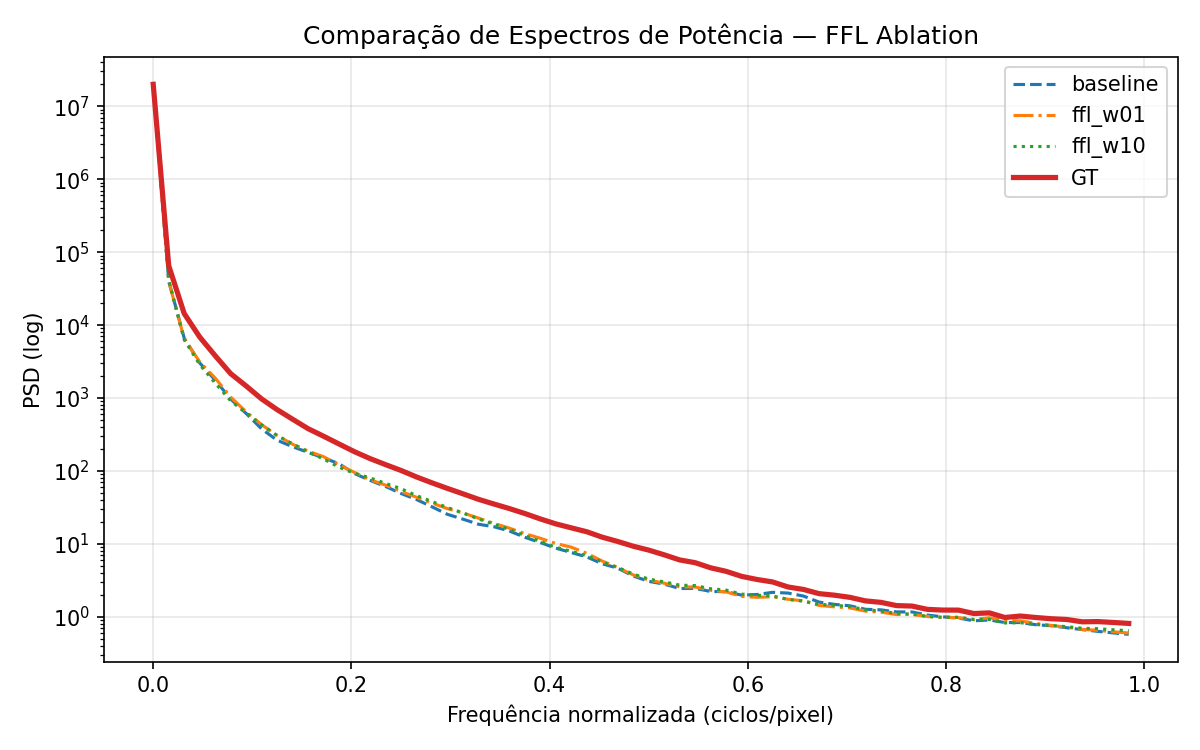
\includegraphics[width=0.85\textwidth]{../resultados/evaluation/psd_comparison.png}
    \caption{PSD radial média (escala log) das três variantes e do \textit{ground truth}.
    Todas as variantes apresentam déficit de energia nas frequências médias--altas
    (0{,}1--0{,}5 ciclos/pixel) em relação ao GT, caracterizando o gap espectral.
    A diferença entre variantes é sutil nesta escala; o PSD\_L2 quantifica
    numericamente a distância ao GT.}
    \label{fig:psd}
\end{figure}

A Figura~\ref{fig:psd} mostra que todas as variantes seguem a mesma tendência:
forte energia nas baixas frequências (estruturas grossas) e queda progressiva
nas altas frequências. O \textit{ground truth} (aerofoto) mantém maior energia
nas frequências intermediárias (detalhes finos como bordas de edifícios, texturas
de vegetação), refletindo a maior resolução espacial do sensor aéreo.

\subsection{Comparação de Métricas por Barra}

\begin{figure}[H]
    \centering
    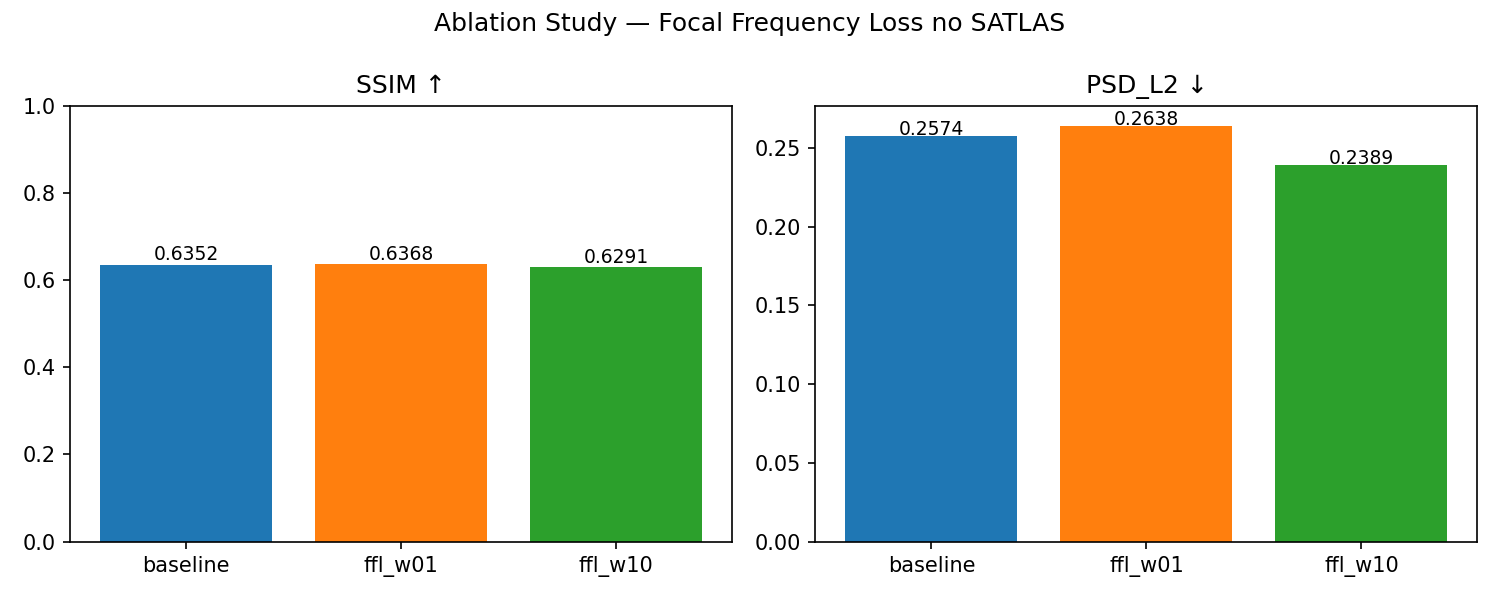
\includegraphics[width=0.85\textwidth]{../resultados/evaluation/metrics_comparison.png}
    \caption{Comparação de SSIM (esquerda) e PSD\_L2 (direita) entre as três
    variantes. FFL $\lambda=1{,}0$ apresenta o melhor equilíbrio espectral
    (menor PSD\_L2) ao custo de leve redução de SSIM.}
    \label{fig:barras}
\end{figure}

\subsection{Discussão}

O resultado é consistente com o mecanismo da FFL. O L1 minimiza o erro
pixel a pixel, o que penaliza erros em baixas frequências (que têm maior
energia e portanto maior contribuição para o MSE) mais do que erros em
altas frequências. Isso produz geradores que recuperam bem a estrutura
grosseira da cena, mas suavizam as texturas finas. A FFL reequilibra esse
gradiente: ao ponderar o erro no domínio de frequências de forma adaptativa,
ela direciona o gerador para recuperar as componentes espectrais ainda mal
aprendidas --- tipicamente as de alta frequência.

O fato de $\lambda=0{,}1$ não produzir melhora sugere que, neste domínio
(Planet $\rightarrow$ aerofoto), o gap espectral é suficientemente grande
para exigir um peso maior de FFL. Com $\lambda=1{,}0$, o gerador efetivamente
``sacrifica'' algum alinhamento estrutural (queda de SSIM) para recuperar
mais energia nas frequências altas (queda de PSD\_L2) --- o \textit{trade-off}
característico de losses espectrais versus espaciais.

% =====================================================================
\section{Conclusões}
% =====================================================================

Este trabalho demonstrou que a adição da Focal Frequency Loss ao \textit{fine-tuning}
do SATLAS com dados Planet $\rightarrow$ aerofoto produz melhora mensurável
na fidelidade espectral da superresolução. Os principais achados são:

\begin{itemize}
    \item \textbf{FFL $\lambda=1{,}0$ reduz o PSD\_L2 em 7{,}2\%} em relação
    ao baseline, confirmando que a loss espectral direciona o gerador para
    recuperar frequências altas suavizadas pelas losses convencionais.

    \item \textbf{O custo de SSIM é pequeno} ($\Delta = -0{,}006$), sugerindo
    que o \textit{trade-off} é favorável em aplicações que priorizam fidelidade
    espectral sobre similaridade estrutural pixel a pixel.

    \item \textbf{$\lambda=0{,}1$ é insuficiente} para o gap Planet--aerofoto,
    indicando que a magnitude do gap determina o peso mínimo efetivo da FFL.

    \item A \textbf{avaliação no domínio de frequências} (PSD\_L2) é essencial
    para quantificar ganhos que métricas espaciais (SSIM, PSNR) não capturam.
\end{itemize}

Como trabalho futuro, propõe-se avaliar pesos intermediários de $\lambda$
(0{,}3, 0{,}5), investigar o efeito de mais dados de treinamento (maior área
geográfica) e comparar com outros métodos de superresolução guiada por frequência.

% =====================================================================
% REFERÊNCIAS
% =====================================================================
\begin{thebibliography}{9}

\bibitem{ffl}
    L.\ Jiang, B.\ Dai, W.\ Wu e C.\ C.\ Loy,
    ``Focal Frequency Loss for Image Reconstruction and Synthesis,''
    \textit{Proceedings of ICCV}, pp.~13919--13929, 2021.
    \url{https://arxiv.org/abs/2012.12821}.

\bibitem{satlas}
    P.\ Wolters, F.\ Bastani e A.\ Kembhavi,
    ``Zooming Out on Zooming In: Advancing Super-Resolution for Remote Sensing,''
    \textit{arXiv:2311.18082}, 2023.
    Código: \url{https://github.com/allenai/satlas-super-resolution}

\bibitem{esrgan}
    X.\ Wang \textit{et al.},
    ``ESRGAN: Enhanced Super-Resolution Generative Adversarial Networks,''
    \textit{Proceedings of ECCV Workshops}, 2018.

\bibitem{basicsr}
    X.\ Wang \textit{et al.},
    ``BasicSR: Open Source Image and Video Restoration Toolbox,''
    2022. Disponível em: \url{https://github.com/XPixelGroup/BasicSR}

\bibitem{planet}
    Planet Labs PBC,
    ``Planet Imagery Product Specifications,'' 2023.
    Disponível em: \url{https://www.planet.com/products/satellite-imagery/}

\bibitem{wang2004ssim}
    Z.\ Wang, A.\ C.\ Bovik, H.\ R.\ Sheikh e E.\ P.\ Simoncelli,
    ``Image Quality Assessment: From Error Visibility to Structural Similarity,''
    \textit{IEEE Transactions on Image Processing}, vol.\ 13, n.\ 4, 2004.

\end{thebibliography}

\end{document}
